% !TEX root = root.tex
\chapter{Dynamical and Mechanical Evolution of Bacterial Biofilms at the Oil--Water Interface}
\chaptermark{Bacterial Biofilms}

\section{\label{sec:intro}Introduction}
When bacteria cells in suspension encounter a bounding surface, they form biofilms comprising adherent cells in a complex matrix of extracellular polymeric substances including polysaccharides and surfactants secreted by the bacteria.\cite{Watnick2000}. On solid surfaces, biofilms are ubiquitous and widely studied.  It has been estimated that 99\% of the world's population of bacteria are found in biofilms in various stages of growth \cite{Garrett 2008,Dalton 1998}.  Biofilms provide important biological functions for the bacteria within them, including protection from antimicrobial agents secreted by competing species or deliberately added to prevent infections \cite{Garrett 2008,Flemming 2010}. Because of this protective property, and the fact that they are notoriously difficult to remove, biofilms often have detrimental consequences. For example, biofilms on medical implants and equipment are often resistant to antibiotics and contribute to the spread of disease. Furthermore, owing to their mechanical toughness, biofilms can disrupt or impede the proper function of wide ranges of equipment, for example, by increasing the drag on ships, by decreasing the efflux from outlets from factories, and by fouling filters and bioreactors\cite{Kokare2009}. Biofilms can also be beneficial, for example, in the context of bioremediation, in which bacteria and the films they create remove toxins from their surroundings. For example, bacteria attach to, metabolize, aggregate and sediment undesirable substances, ranging from WHAT to WHAT  aiding wastewater treatment\cite{GuellideSouza2012}. A variety of bacteria are known to biodegrade alkanes, and are exploited in the cleaning of soils and sands contaminated by oil\cite{Rosenberg1985}. The microstructure of the biofilms resembles, from a physical perspective, a disordered colloidal suspension in a polymer solution. The evolution, structure, and mechanics of biofilms on solid surfaces are relatively well studied, including studies of the rate of attachment and its dependence on flow environment\cite{Stoodley1998}, the rheology\cite{Klapper2002} and microrheology of the films\cite{Rogers2008} and changes to cell physiology\cite{Wilking2011}. The study of biofilm structure and function continues to reveal important insights into issues ranging from the evolutionary advantages of cooperation, (REF) to strategies for displacement of colonies by competing species which rely on invasion of  motile cells into biofilms which impart transient biofilm permeability\cite{Houry2012}.

Bacteria also form biofilms at fluid interfaces; the stages of growth of these films and their mechanics are less studied.  At air-aqueous interfaces, biofilms have been studied in terms of their rate of growth and their micromechanics, motivated in part by interest in cystic fibrosis lung infections and the behavior of airborne infectious agents\cite{Wu2012}. These studies help reveal biofilm microstructure\cite{Fuller2012} and inform strategies to manipulate them.  Biofilms at oil-water studies have also been studied, in part motivated by bioremediation of oil spills. Natural blooms of bacteria occur in the presence of spilled oil, and much has been done to increase the speed and ability of the bacteria to degrade pollutant hydrocarbons\cite{Abbasnezhad2011, Warr2013}. 

The ability of bacteria to attach to oil-aqueous interfaces is well documented.  One widely used assay, with acronym BATH/MATH for bacterial or microbial adhesion to hydrocarbons relies on optical density measurements of aqueous phases to quantify depletion of microbes from suspension containing dispersed droplets of hydrocarbons, and to thereby infer the adsorption of microbes to oil/water interfaces\cite{Rosenberg1985}. More direct methods involve imaging oil-water interfaces and directly visualizing the microbes as they attach to the interface.

The external surfaces of bacteria are highly complex, presenting surface structures such as pili, lipopolysaccharide O antigen or teichoic acid, and exopolysacchafides\cite{Dalton1998}. The wide range of surface chemistries and structures presented on the bacterial surfaces and their varying shapes strongly affect their ability to adhere and subsequently degrade oil. Interfacial adhesion has been found to play an important role in bacterial bioremediation of sparingly soluble hydrocarbons\cite{Abbasnezhad2011}. Immediately after encountering a bounding surface, bacteria can remain motile. Bacteria at solid-fluid interfaces have been documented to behave differently than those at fluid-fluid interfaces, for example exhibiting counterclockwise circular motion at an air-water interface, and clockwise circular motion on glass surfaces\cite{Lemelle2010}.  In systems with surfactant producing bacteria, there is contention regarding the behavior of the secretions; one study described an immobilization of the interface, where another suggested that the surfactants contributed to superdiffusion at the air-water interface\cite{Beer2011}.

Here, we study the time evolution of bacterial biofilms at and near planar oil-water interfaces by tracking the mobility of passive colloidal tracers at the interface. This work was part of a wider study of these films that also included biofilms on pendant drops of oil suspended in bacterial suspension in collaboration with the Stebe group at U. Penn. Here, I report only on the particle tracking part of the study, in which I played a lead role working with Liana Vaccari and Aayush Singh. I will also mention briefly the findings of the pendant drop study for context.

The particle tracking and pendant drop experiments together reveal three stages of biofilm evolution. Initially, the preponderance of bacteria near the interface are highly motile, and we refer to this as an ``active'' layer. Over time, a biofilm of adherent bacteria trapped in the interface forms; in the absence of nutrient addition, these bacteria are non-motile. At this stage, the biofilm is viscoelastic. We discuss the implications of this work from a fundamental perspective, as a quasi-two-dimensional, active, glassy system.  Finally, the biofilm becomes an rigid ``skin'' that wrinkles upon compression.

\section{\label{sec:methods}Experimental Methods}
\subsection{Sample Preparation}
Pseudomonas sp. ATCC 27259, strain P62 was chosen as a model organism. Bacteria were cultured in ATCC Medium:3 Nutrient Broth in 24 ppt Instant Ocean to simulate a middle level marsh salinity. The cultures were grown on a table-top shaker at 150 rpm at room temperature for ~24 h to mid-to-late exponential phase. In the biofilm characterization experiments, a bacteria suspension free of surface active proteins from the nutrient broth was prepared with a typical washing protocol (Rosenberg, Kang, Klein) by centrifuging the culture for 5 minutes at 5000 x g, decanting the nutrient broth or supernatant and re-suspending the pellet in Instant Ocean three times. Control microrheology experiments of dilute nutrient broth were performed absent bacteria to confirm the evolution of the interface was due to bacteria and biofilm development.
\subsection{Particle Tracking}
The particle-tracking measurements are performed in a 1.0 cm ID cylindrical vessel with an inner surface whose bottom half is aluminium and top half is Teflon.  When the cell is filled to the appropriate level, the aluminum-Teflon seam pins the oil-water interface, creating a flat surface with no meniscus. The base of the cylinder rests on an untreated glass coverslip, sealed by a PDMS gasket.  To begin each experiment, the cylinder is filled nearly to the seam with 0.5 ml of Instant Ocean.  A spreading solution containing charge-stabilized polystyrene spheres (Interfacial Dynamics Corp.) with radius Rs = 0.5 ?m in a mixture of equal parts by volume water and isopropanol is prepared in advance and sonicated to disperse any colloidal aggregates.  To introduce the colloids to the interface, a 10-?L droplet of the spreading solution is gently placed in contact with the Instant Ocean surface.  The solution wets the surface, and the colloids, slightly denser than water but hydrophobic, disperse across the surface. Droplets of hexadecane are then promptly applied to the surface until it is completely covered.  The age of the sample ta is measured from this instant of interface formation.  After each experiment, the cylindrical vessel is cleaned thoroughly by scrubbing and sonicating in Alconox soap solution, acetone, and isopropanol, and then rinsed repeatedly in deionized water.
We observe the colloids at the interface using an upright bright-field microscope with a 50x objective.  A camera (Zeiss AxioImager M1m) records a 200-?m by 150-?m field of view at 60 frames per second, which set the shortest lag time over which probe motion can be characterized.  Probe trajectories are extracted from the video using a custom Python implementation (Allan Keim Caswell, in prep) of the widely used Crocker-Grier multiple-particle-tracking algorithm\cite{Crocker1996}. Static and dynamic errors in the particle tracking are accounted for to avoid distortion in the measurements of particle trajectories\cite{Savin2005}. Trajectories are extracted from video segments short enough in duration (typically 1-2 minutes) so that no apparent change in particle mobility due to the evolving interfacial properties can be discerned over the selected time span. Typically 30-200 probes are in view at a time, constituting at most 0.3\% surface coverage.  
\section{Results}
The interface between hexadecane and the seawater bacteria solution evolves with age, changing measurably over a timescale of minutes. We discuss three qualitatively distinct stages of the biofilm development during which it can be characterized as (i) active, (ii) viscoelastic, and finally (iii) rigid.  The first two stages of development are investigated primarily through the particle-tracking experiments, while the third stage of biofilm rigidity is characterized using the pendant drop experiments.
\subsection{Tracer Motion at an Active Interface}
Immediately following the formation of a fresh interface between the oil and bacteria suspension, bacteria were sometimes observed to associate with the interface and remain motile once attached. Bacteria attach to the interface in both end-on and side-on orientations. Often, bacteria at the surface were accompanied by a population of especially mobile bacteria just beneath the interface.  In these cases, the colloidal motion at the interface was strongly affected by hydrodynamic interactions with the swimming bacteria at the surface and by direct collisions with those at the surface. Typically, the concentration of swimming bacteria embodied a 10\% area fraction of the interface�large enough to lead to collective motion such as swirling, which influenced the colloidal motion. A substantial literature has addressed the mobility of colloidal probes in the presence of motile bacteria and other microbial swimmers both in bulk (3D) and in quasi-two-dimensional contexts\cite{Wu2000,Dombrowski2004,Wilson2011,Soni2003a,Chen2007,Mino2011a,Jepson2013,Leptos2009,Rushkin2010,Kurtuldu2011}. One motivation for studying the colloidal dynamics in suspensions of swimming microbes is their utility as model systems for investigating the nonequilibrium statistic mechanics of active complex fluids.  In addition, the colloid motion provides insight into biomixing, the enhanced transport of nutrients and other material by active suspensions. Since biofilm formation relies on the transport of polysaccharides and other constituents to and within the interface, such biomixing could be an important feature of the film development. Hence, we have characterized the colloidal motion during this active phase in some detail.

\begin{figure}[htbp]
  \centering
  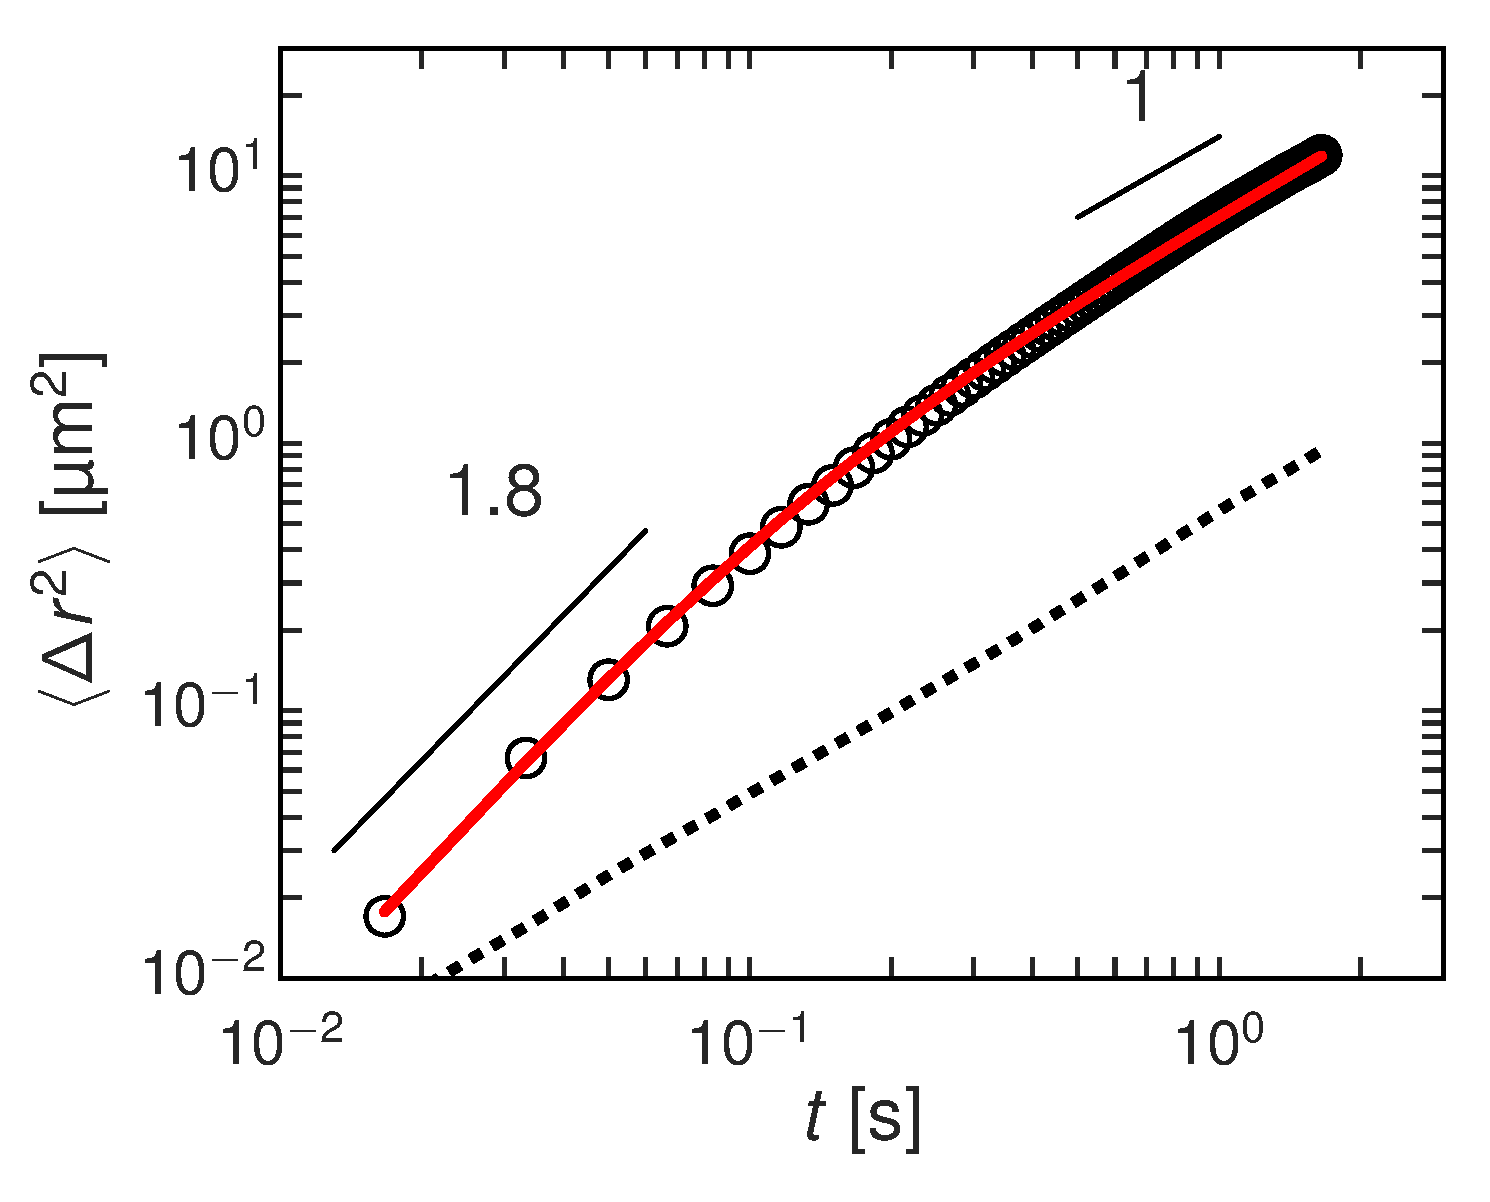
\includegraphics[width=\columnwidth]{bacteria/R1-active-msd}
  \caption{Ensemble-average mean-squared displacement of colloidal tracers during the initial, active stage of biofilm formation at an oil-water interface.  For reference, the dashed line displays the mean-squared displacement of colloids at the oil-water interface in the absence of bacteria.  The solid line displays the result of a fit using Eq. \ref{eqn:mss-memory}.}
  \label{fig:R1}
\end{figure}

Figure \ref{fig:R1} shows the colloids� ensemble-average mean-squared displacement, $\langle \Delta r^2 (t)\rangle = \langle(\vec{r}_i (t' + t) - \vec{r}(t')\rangle_{i, t'}$where the average is over particles i and time t�, during this active stage of biofilm formation.  For reference, the mean-squared displacement of colloids at the oil interface of pure Instant Ocean containing no bacteria is also shown.  In the absence of bacteria, $\langle \Delta r^2 (t) \rangle$ varies linearly with lag time t indicating simple diffusion, $\langle \Delta r^2 (t) \rangle=4D_0 t$, with a diffusion coefficient, $D_0 = 0.12 \mu m^2/s$, consistent with the viscosities of water and hexadecane.  The mean-squared displacement of the colloids at the active interface similarly varies linearly with t at large lag times, but with an enhanced effective diffusion coefficient.  At smaller lag times, the mean-squared displacement grows more rapidly than linearly, indicating superdiffusive motion.  Such superdiffusive motion is a common feature of colloidal motion in microbial suspensions and signals temporal correlations in the forcing of the colloids due to hydrodynamic interactions with the swimmers.  A simple model for these correlations ascribes to them a single characteristic correlation time ?, so that the particle velocities have an exponentially decaying memory, $\vec{v}(t')\cdot\vec{v}(t' + t)\sim \exp(-t/\tau)$\cite{Wu2000}.  Such velocity correlations lead directly to a mean-squared displacement of the form \cite{Kurtuldu2011}

\begin{equation}
\langle \Delta r^2 (t) \rangle = 4D\left[t + \tau(e^{-t/\tau} - 1)\right]
\label{eqn:mss-memory}
\end{equation}

\noindent In the limit of short lag times, t << ?, this form predicts ballistic motion, $\langle \Delta r^2 (t) \rangle=\frac{2D}{\tau}t^2$; and at large lag times it reduces to diffusive motion, $\langle \Delta r^2 (t) \rangle=4Dt$, with effective diffusion coefficient $D$.   The solid line in Fig.\ref{fig:R1} is the result of a fit using this form, which describes data accurately and gives $D =1.8�0.1 \mu m^2/s$ and $\tau = 0.053 \pm 0.007$ s.   The value of $D$ in relation to the diffusivity in the absence of bacteria, $D/D_0\approx15$, indicates that biomixing strongly influences the interface during this early stage of biofilm formation.  We note further that this factor likely underestimates the enhancement in tracer mobility due to the swimming bacteria since, as described below, even at these early interface ages the incipient biofilm imparts an interfacial viscosity that reduces thermal diffusivity.

The success of Eq. (\ref{msd-memeory}) in capturing the form of $\langle \Delta r^2 (t) \rangle$ is consistent with several earlier studies of colloidal motion in active microbial suspensions and hence indicates that the velocities of tracers in such suspensions indeed have exponentially decaying memory.  However, we can interrogate these correlations more directly by defining an instantaneous direction of motion for each particle,

\begin{equation}
\hat{n}(t) = \frac{\vec{r}_i(t) - \vec{r}_i(t + \delta t)}{|\vec{r}_i(t) - \vec{r}_i(t + \delta t)|}
\end{equation}

\noindent where $\delta t = 1/60$ s is the time between successive video frames and $i$ labels the particles, and by examining its time-time autocorrelation function,

\begin{equation}
\Phi_n(t) = \langle\hat{n}_i(t + t')\cdot\hat{n}_i(t)\rangle_{i,t'}
\end{equation}

\begin{figure}[htbp]
  \centering
  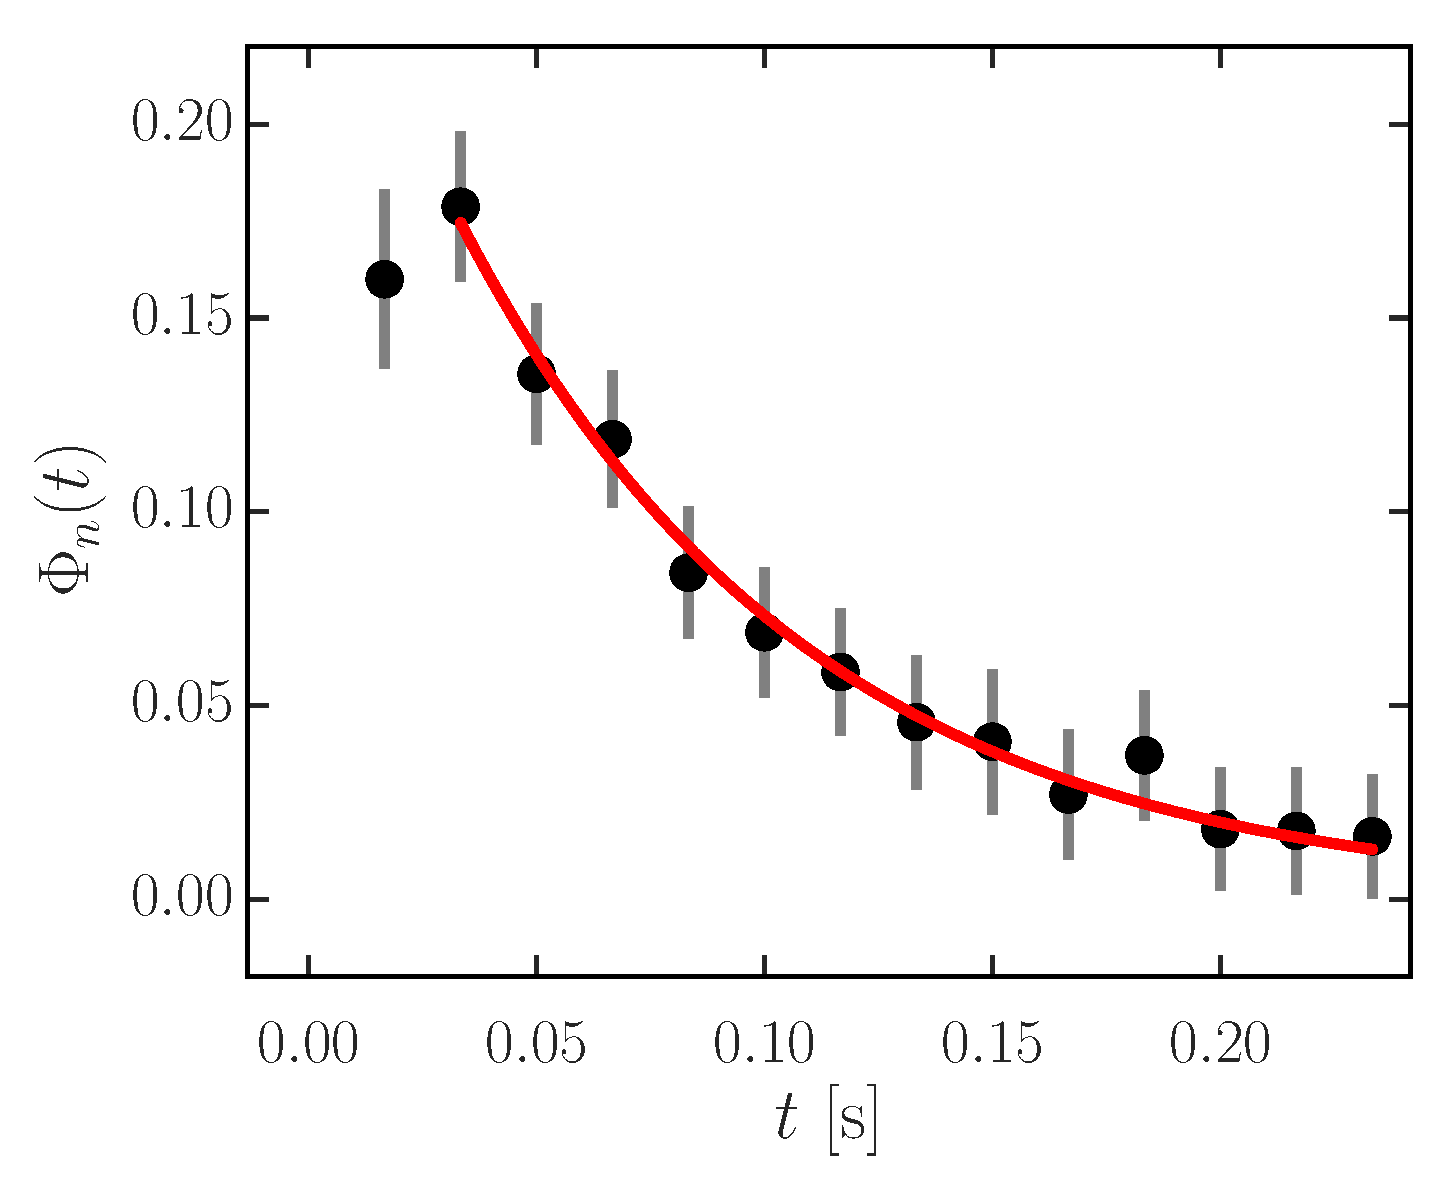
\includegraphics[width=\columnwidth]{bacteria/R2-time-autocorrelation}
  \caption{Time autocorrelation function of the direction of instantaneous tracer displacements during the active stage of biofilm formation.  The line shows the result of an exponential fit to the data at large times ($t > 0.03$ s).}
  \label{fig:R2}
\end{figure}

The significance of $\Phi_n (t)$ is that it quantifies the persistence in the direction of the colloids� trajectories.  As shown in Fig. \ref{fig:R2}, $\Phi_n (t)$ is effectively zero at $t > 0.15$ s, setting the typical time required for the colloids� direction of motion to randomize completely.  Notably, $\Phi_n (t)$ does not decay monotonically but has a peak near $t = 0.03 $s.  We attribute this peak to a tendency for colloids to follow ``U-shaped'' trajectories on short time scales due to hydrodynamic interactions with bacteria swimming past in close proximity\cite{Leptos2009}, and hence to make negative contributions to $\Phi_n (t)$.  At larger times, $\Phi_n (t)$ decays exponentially, as shown by the line in Fig. \ref{fig:R2}, which is an exponential fit to the data.  The correlation time obtained from the fit is $0.075 \pm 0.01$ s, which is in reasonable agreement with the characteristic time $\tau$ for velocity correlations implied by fitting $\langle \Delta r^2 (t)\rangle$ with Eq. (\ref{msd-memory}).  Thus, through $\Phi_n (t)$ we observe directly the nature of the correlated tracer dynamics in an active suspension inferred by the analysis of $\langle \Delta r^2 (t)\rangle$.

\begin{figure}[htbp]
  \centering
  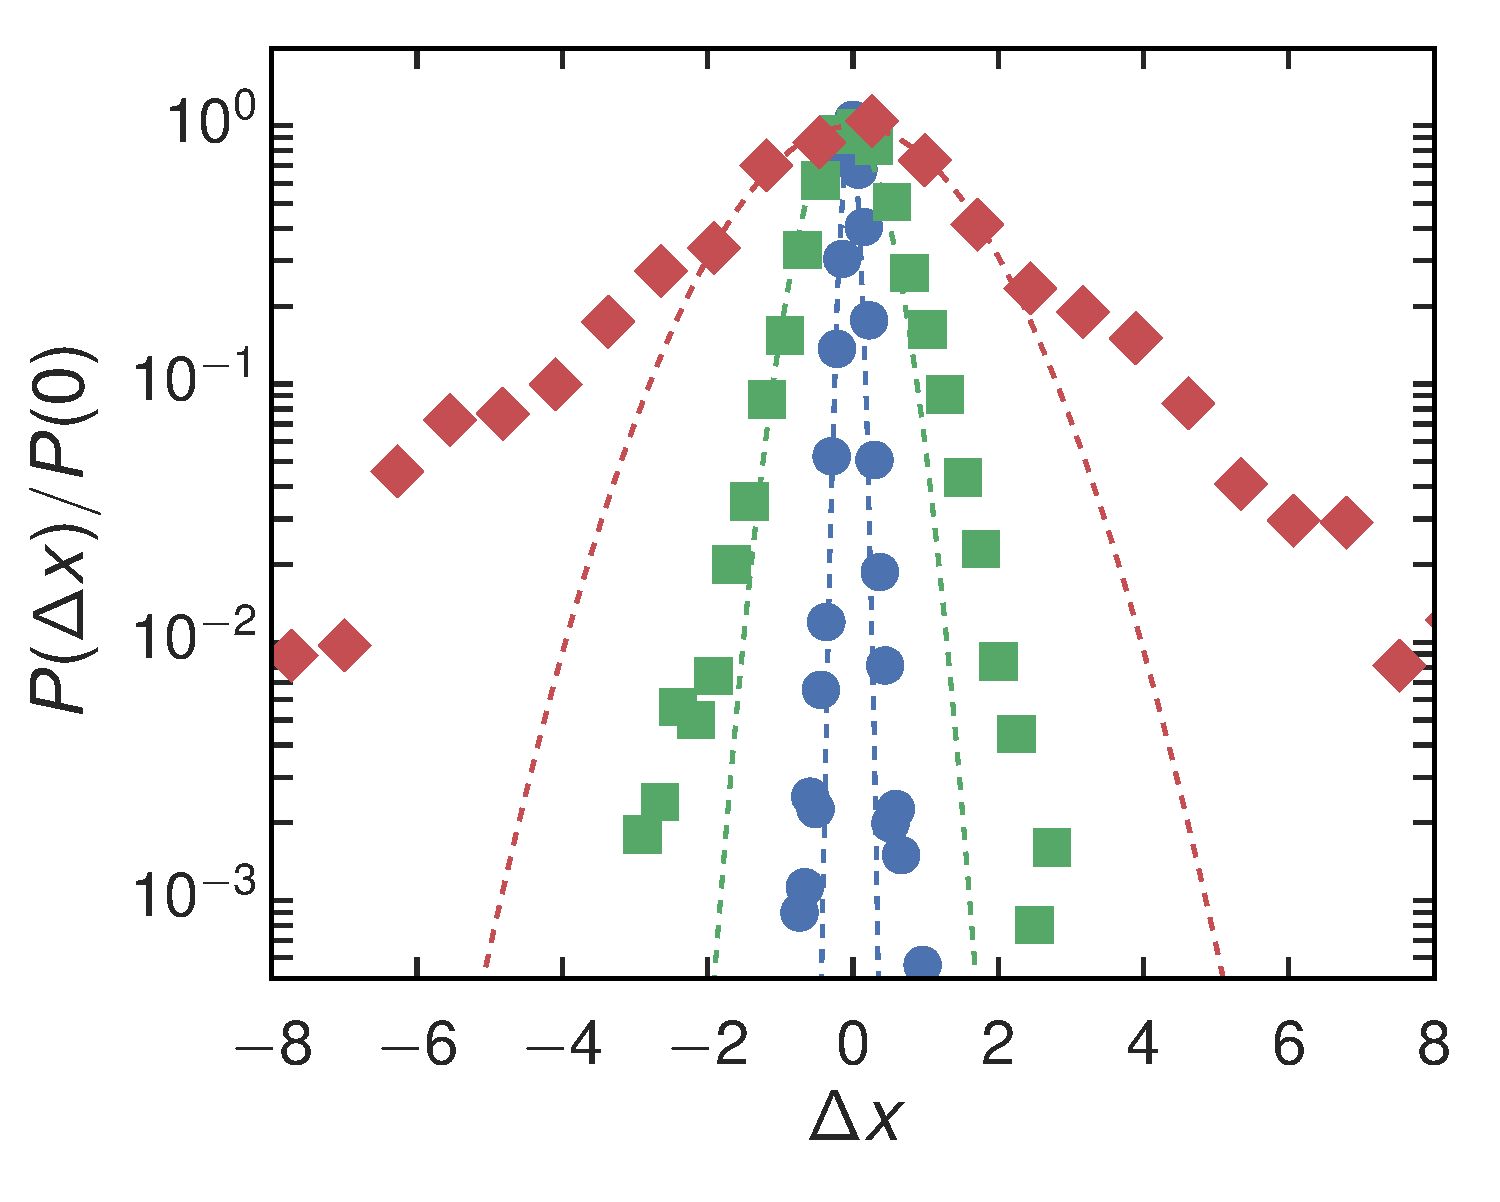
\includegraphics[width=\columnwidth]{bacteria/R3-Active-nongaussian-van-Hove}
  \caption{Normalized probability distribution functions for colloidal displacements at lag times of 0.016 s (blue), 0.15 s (green), and 1.3 s (red) during the active stage of biofilm formation.  The solid lines display the results of fitting Gaussian lineshapes in the regions of the peaks of the distributions, highlighting the enhanced, non-Gaussian probability for large displacements.}
  \label{fig:R3}
\end{figure}


While the colloids� Brownian dynamics at large lag times with diffusivity $D$ suggest that the suspension of swimming bacteria act like a thermal bath with large effective temperature, several previous studies have emphasized that the statistical properties of the colloidal displacements differ from those expected for a system in thermal equilibrium \cite{Chen2007,Leptos2009,Kurtuldu2011}.  These differences are apparent in the probability distribution function (PDF) for displacements at fixed lag time $P_t (\Delta x)$, where $\Delta x$ is the displacement along one direction.  Figure \ref{fig:R3} shows $P_t (\Delta x)$ at $t = 0.0167$ s, 0.15 s, and 1.3 s, lag times spanning the superdiffusive and diffusive behavior in $\langle \Delta r^2 (t)\rangle$.  The PDFs of particles undergoing thermal diffusion in equilibrium would be Gaussian.  In all cases, the PDFs in the active, incipient biofilm show clear deviations from Gaussian forms, with tails at large $|\Delta x|$ that signal enhanced probability of large displacements.  Qualitatively similar non-Gaussian PDFs have been observed previously among tracers in microbial suspensions and have been associated with advection-enhanced large displacements due to hydrodynamic encounters between the colloids and swimmers\cite{Leptos2009,Kurtuldu2011}.  To compare the form and magnitude of the non-Gaussian contributions to $P_t (\Delta x)$ at different lag times more closely, we plot in Fig. \ref{fig:R4} the normalized PDFs with displacement normalized by the root mean-squared displacement.  Remarkably, the normalized PDFs collapse onto a single lineshape, indicating that the distribution function maintains a self-similar form with increasing lag time.  Such self similarity is generally unexpected and implies particular attributes about the colloidal dynamics, including (i) that the fraction of colloids in the non-Gaussian population remains constant over the range of lag times probed, and (ii) that the Gaussian and non-Gaussian displacements grow as the same function of lag time, first superdiffusively at short lag times and then diffusively at longer lag times.  Self-similar distributions with non-Gaussian tails were also observed among tracer displacements within bulk (3D) suspensions of the eukaryotic microorganism Chlamydomonas\cite{Leptos2009}.  However, in that case, $\langle \Delta r^2 (t)\rangle$ displayed diffusive behavior over the entire range of lag times probed.  The collapse in Fig. \ref{fig:R4} is particularly notable because the lag times span both the superdiffusive and diffusive regimes.  In both the previous case of tracers among swimming Chlamydomonas and in our case of tracers in an incipient biofilm, the non-Gaussian contributions to the probability distribution function follow a Laplace distribution, so that the total PDF can described as the sum of two parts,

\begin{equation}
\label{eq:gaussian-laplacian}
P(\Delta x) = \frac{1 - f}{\sqrt{2\pi\sigma^2}}\exp\left[-\frac{1}{2}\frac{\Delta x}{\sigma}^2\right] + \frac{f}{\xi}\exp\left[-\frac{|\Delta x|}{\xi}\right]
\end{equation}

\noindent The solid line in Fig. \ref{fig:R4} is the result of a fit to the data using this form.

\begin{figure}[htbp]
  \centering
  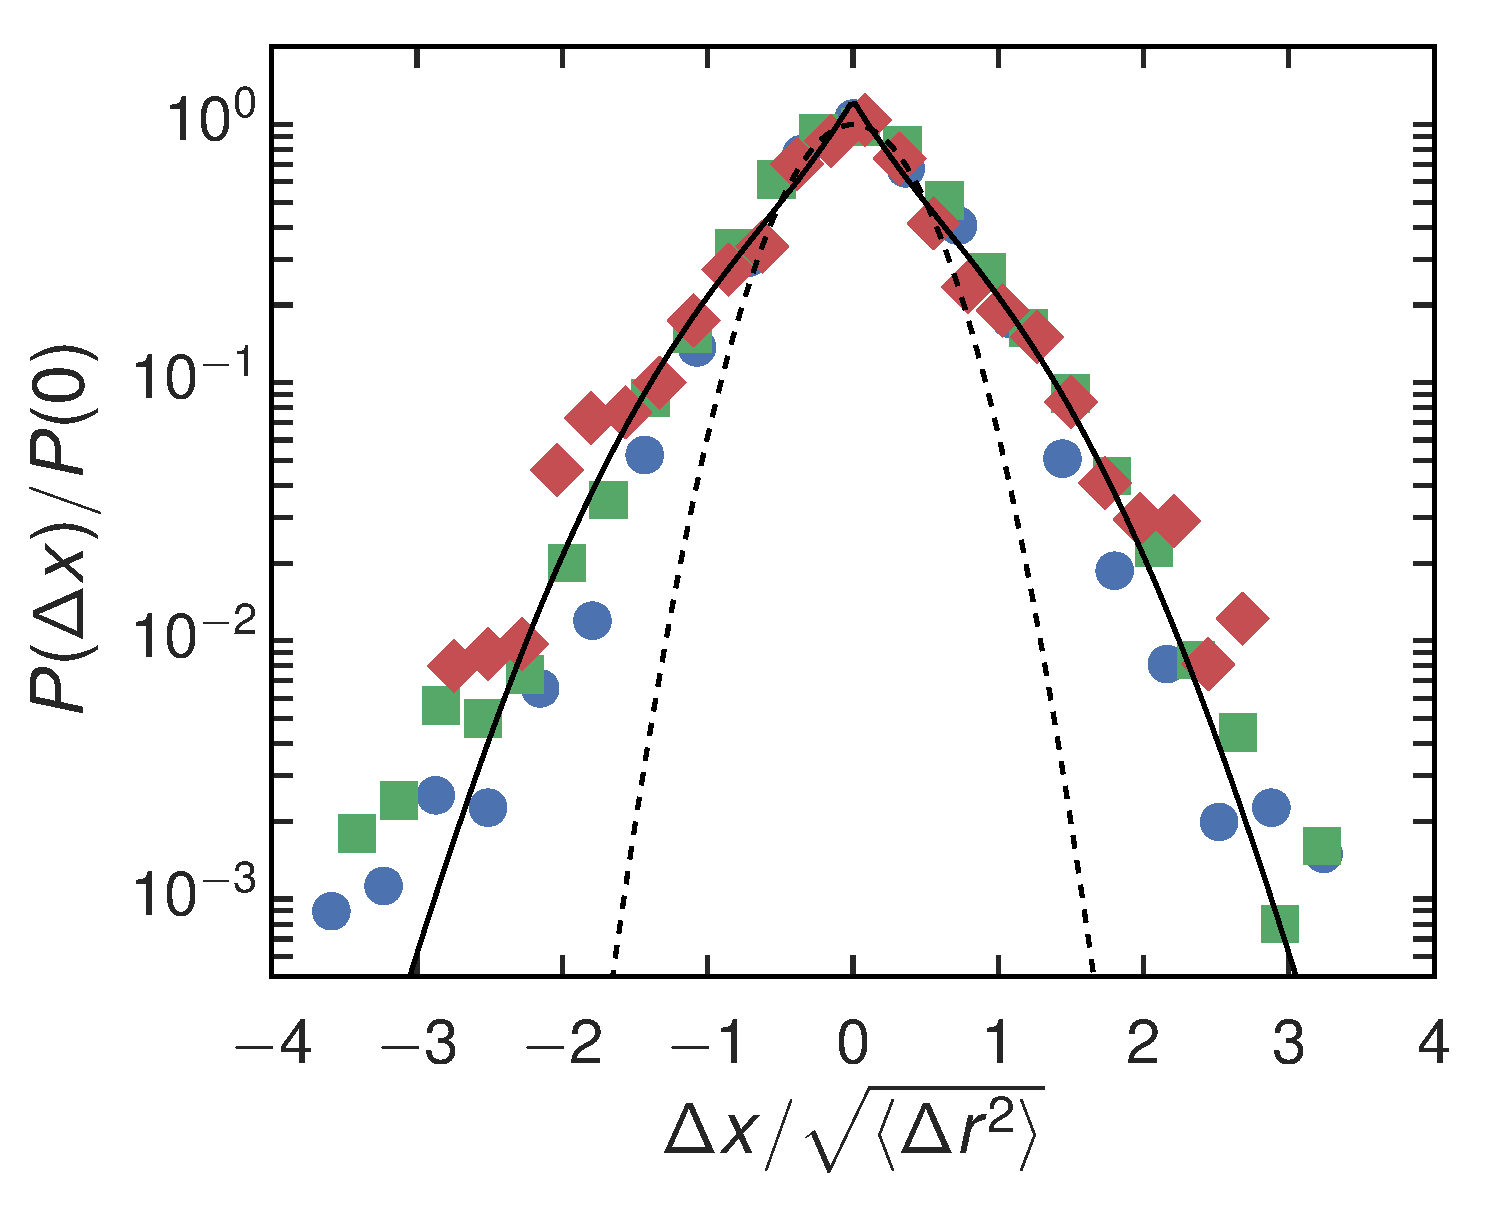
\includegraphics[width=\columnwidth]{bacteria/R4-Active-nongaussian-van-Hove-rescaled}
  \caption{Normalized probability distribution functions from Figure \ref{fig:R3} plotted against displacement normalized by the root mean squared displacement at each lag time, illustrating the collapse of the distributions onto a common lineshape.  The dashed line displays the result of fitting a Gaussian lineshape in the regions of the peak.  The solid line displays the result of a fit using the form given by Eq. \ref{eqn:gaussian-laplacian}}
  \label{fig:R4}
\end{figure}

The strong similarity between the self-similar PDFs of tracer displacements in the incipient interfacial bacterial biofilm and those in bulk suspensions of Chlamydomonas is surprising since the tracer displacements in quasi-2D films of the Chlamydomonas suspensions display qualitatively different non-Gaussian distributions, and the authors of those studies attributed the difference to the differing fluid velocity fields generated by the force dipoles of the Chlamydomonas swimming in two and three dimensions\cite{Kurtuldu2011}.   Our case of colloids entrained at an oil interface of a suspension of swimming bacteria that are forming a biofilm has several features that distinguish it from these studies.  First, the colloids, while in the incipient biofilm, were in contact with the aqueous subphase and hence were coupled hydrodynamically to bacteria both in the film and in the bulk, a situation that is in some sense a hybrid of the three-dimensional and quasi-two-dimensional systems considered previously.  Second, as discussed below, biofilm formation substantially impacts the rheology of the interface even at the earliest ages, with possible qualitative consequences on the coupling between the swimming bacteria and the colloidal tracers in the film.  Finally, Chlamydomonas is a ``puller'' while Pseudomonas sp. is a ``pusher,'' and this distinction has consequences for the collective behavior and resulting hydrodynamics of suspensions.  Given these distinctions, the strong correspondence between the PDFs in Fig. \ref{fig:R4} and those from bulk Chlamydomonas suspensions suggests that such self-similar distributions with Gaussian and Laplacian components might emerge more generically in nonequilibrium active systems than previous thought.

\begin{figure}[htbp]
  \centering
  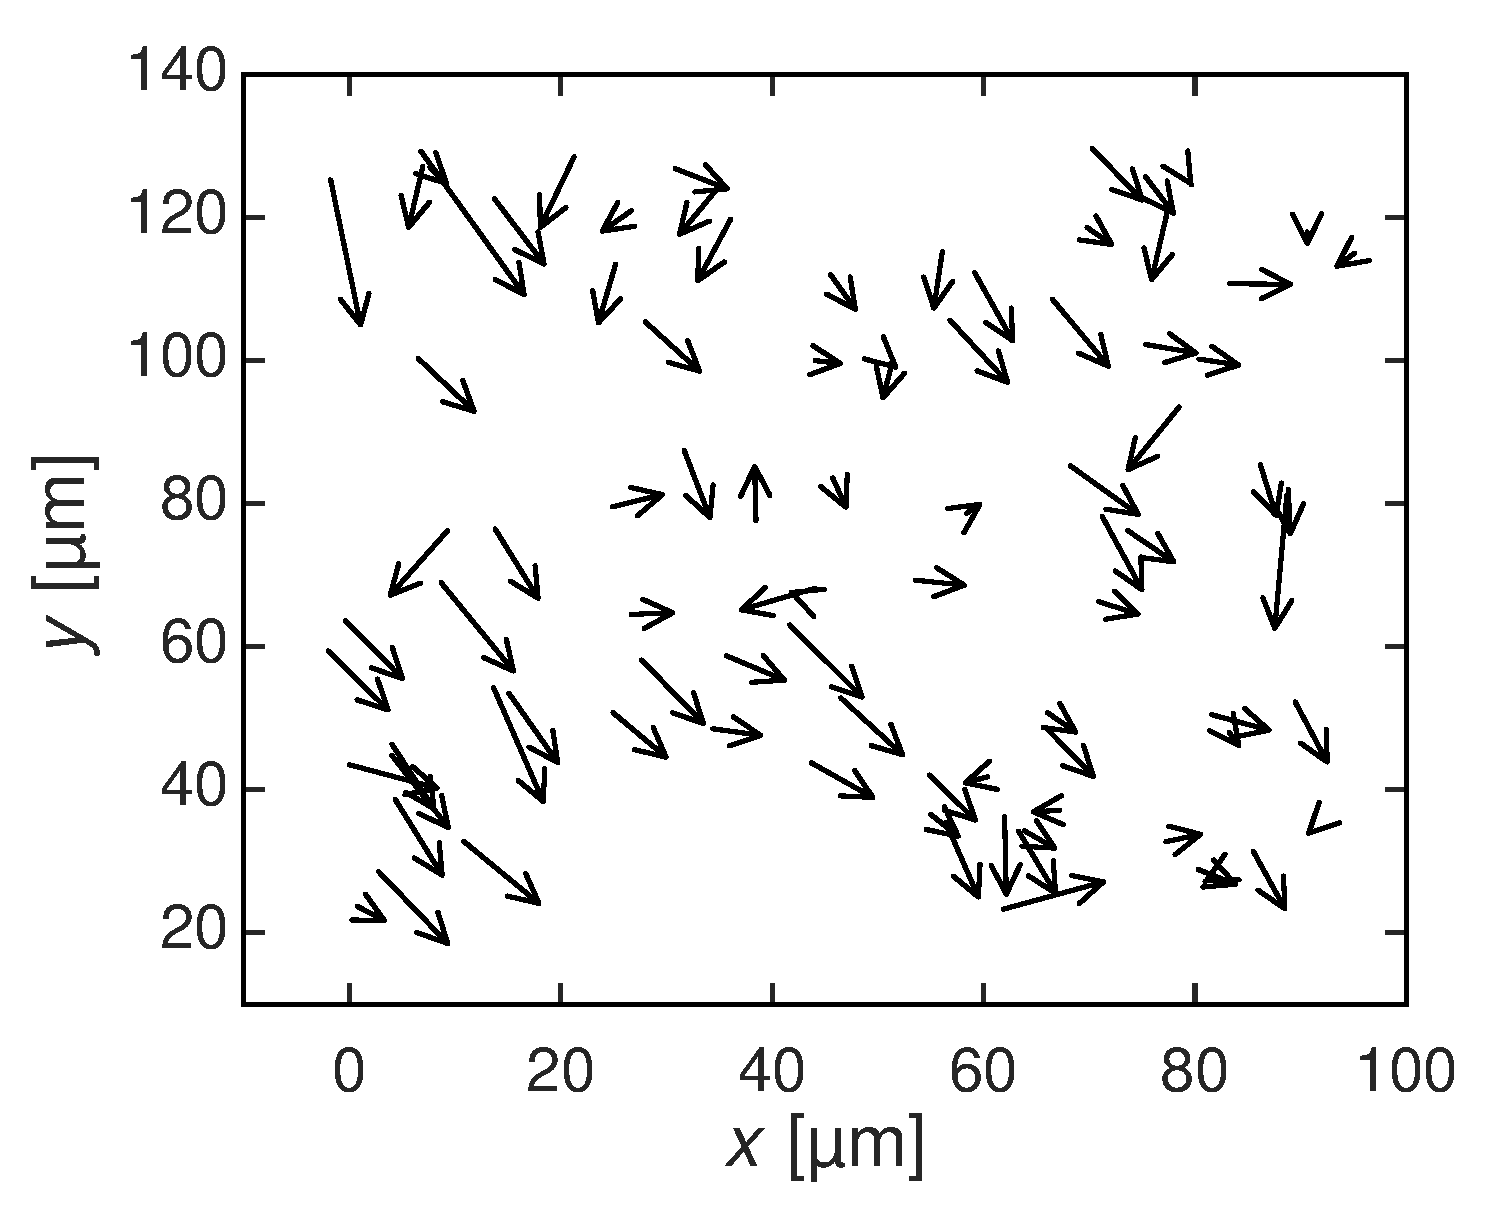
\includegraphics[width=\columnwidth]{bacteria/R5-displacement-arrows}
  \caption{Map of a section of the interface during the active stage of biofilm formation showing the direction of motion of the colloidal tracers at an instant in time. Each colloid is represented by an arrowhead indicating its instantaneous motion $\vec{r}$.}
  \label{fig:R5}
\end{figure}

Another feature of our study of the active stage was the density of colloidal probes at the interface, which was large enough that correlated motion among the colloids could be observed, thereby providing information about the spatial correlations of the non-Brownian �kicks� the swimming bacteria impose.  As an illustration, Figure \ref{fig:R5} depicts $\vec{r}$ for the colloids in the microscope field of view at one instant during the active stage.  Alignment between the direction of motion of nearby colloids is clearly apparent.  This coordinated motion is quantified in Fig. \ref{fig:R6}, which shows the normalized pair direction-direction correlation function,

\begin{equation}
C_n(r) = \langle \hat{n}_i\cdot\hat{n}_j\rangle_{i,j,t}
\end{equation}

where the brackets represent an average over all pairs of particles $i, j$ separated by distance $r$. The spatial correlations in tracer motion decay exponentially with separation, as depicted by the dashed line in Fig. \ref{fig:R6}, which is the result of an exponential fit to the data with correlation length of  $4.7 \pm 1.7 ?m$.  Together, $G_n (t)$ and $C_n (r)$ give a quantitative picture of the short-time, spatiotemporal correlations in tracer motion that characterize the dynamical behavior of the interface during the initial, active stage of biofilm development. 

\begin{figure}[htbp]
  \centering
  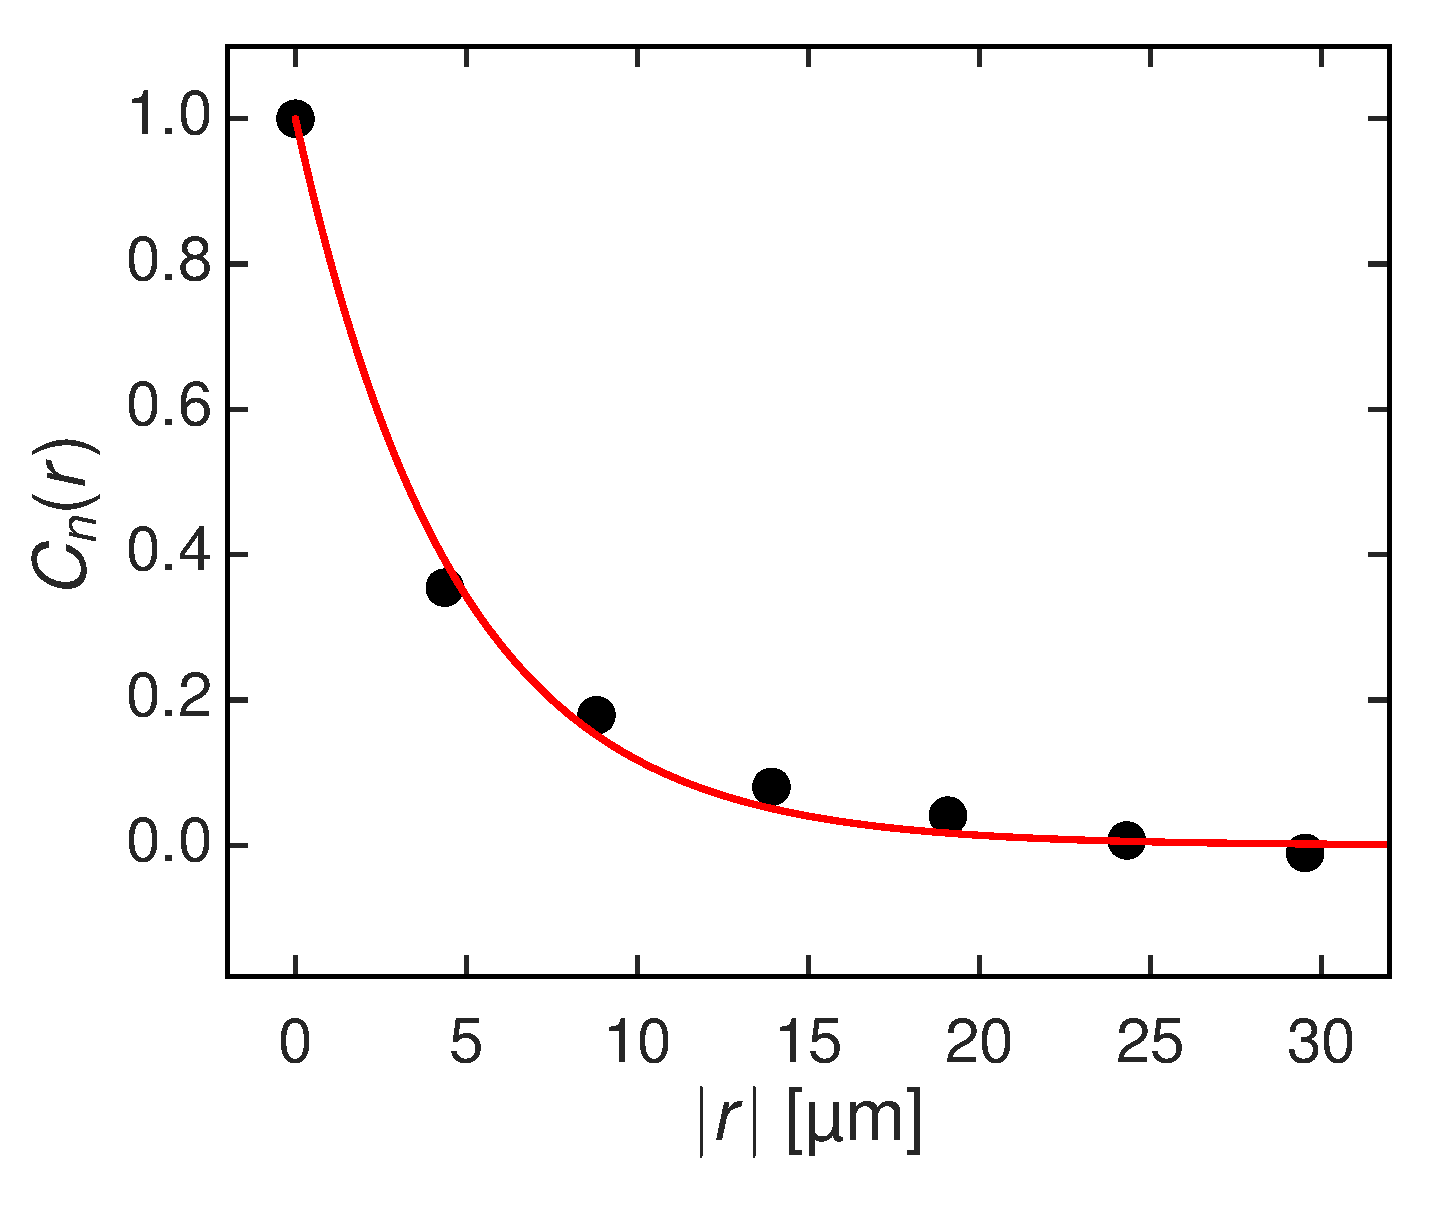
\includegraphics[width=\columnwidth]{bacteria/R6-Cn}
  \caption{Normalized pair direction-direction correlation function as a function of the distance between colloids during the active stage of biofilm development.}
  \label{fig:R6}
\end{figure}

\subsection{Viscoelastic Transition}

Typically, the initial active stage of the biofilm persisted for less than 5 minutes, after which no motile bacteria were observed either at the surface or in the near-surface bulk.  We ascribe the limited duration of the bacteria motility to the lack of nutrient in the suspension.  The end to the active stage was reflected in a qualitative change to the probe dynamics in which the probe mean-squared displacement changed from superdiffusive at short lag times to subdiffusive.  Once the bacteria ceased to move visibly, we treated the interface as a passive system close to thermodynamic equilibrium and considered the probes to be undergoing thermally-driven Brownian trajectories from which the film rheology could be inferred.

 As mentioned above, the active stage was not always observed.  Significantly, the ensuing mechanical changes of the interface, as inferred from probe mobility, appeared qualitatively independent of whether it was preceded by an active stage. Furthermore, as discussed below, the evolution in film rheology persisted for many minutes after the end of the active stage, suggesting that the presence of absence of an active stage had limited impact on subsequent biofilm evolution.  From these observations we conclude that the film formation was primarily the consequence of polysaccharides and surface-active moieties produced by the non-motile (resting?) bacteria.  However, we cannot discount the possibility of some subtle effects to biofilm formation due to biomixing by the swimming bacteria in those instances with an active stage.
 
Here, we present results for the viscoelastic evolution of the biofilm from an experiment in which no protracted active stage was visible at the start of film formation.  We focus on this data set because (i) the population of (non-motile) bacteria at the interface was limited, leaving a relatively unobstructed interface for the colloids and facilitating the analysis of their Brownian motion, and (ii) the colloidal motion was less likely to be affected by any residual activity than in a trial with a fully realized active stage.  We emphasize again that the trends observed were qualitatively the same as those in trials in which the viscoelastic film development was preceded by an active stage.

\begin{figure}[htbp]
  \centering
  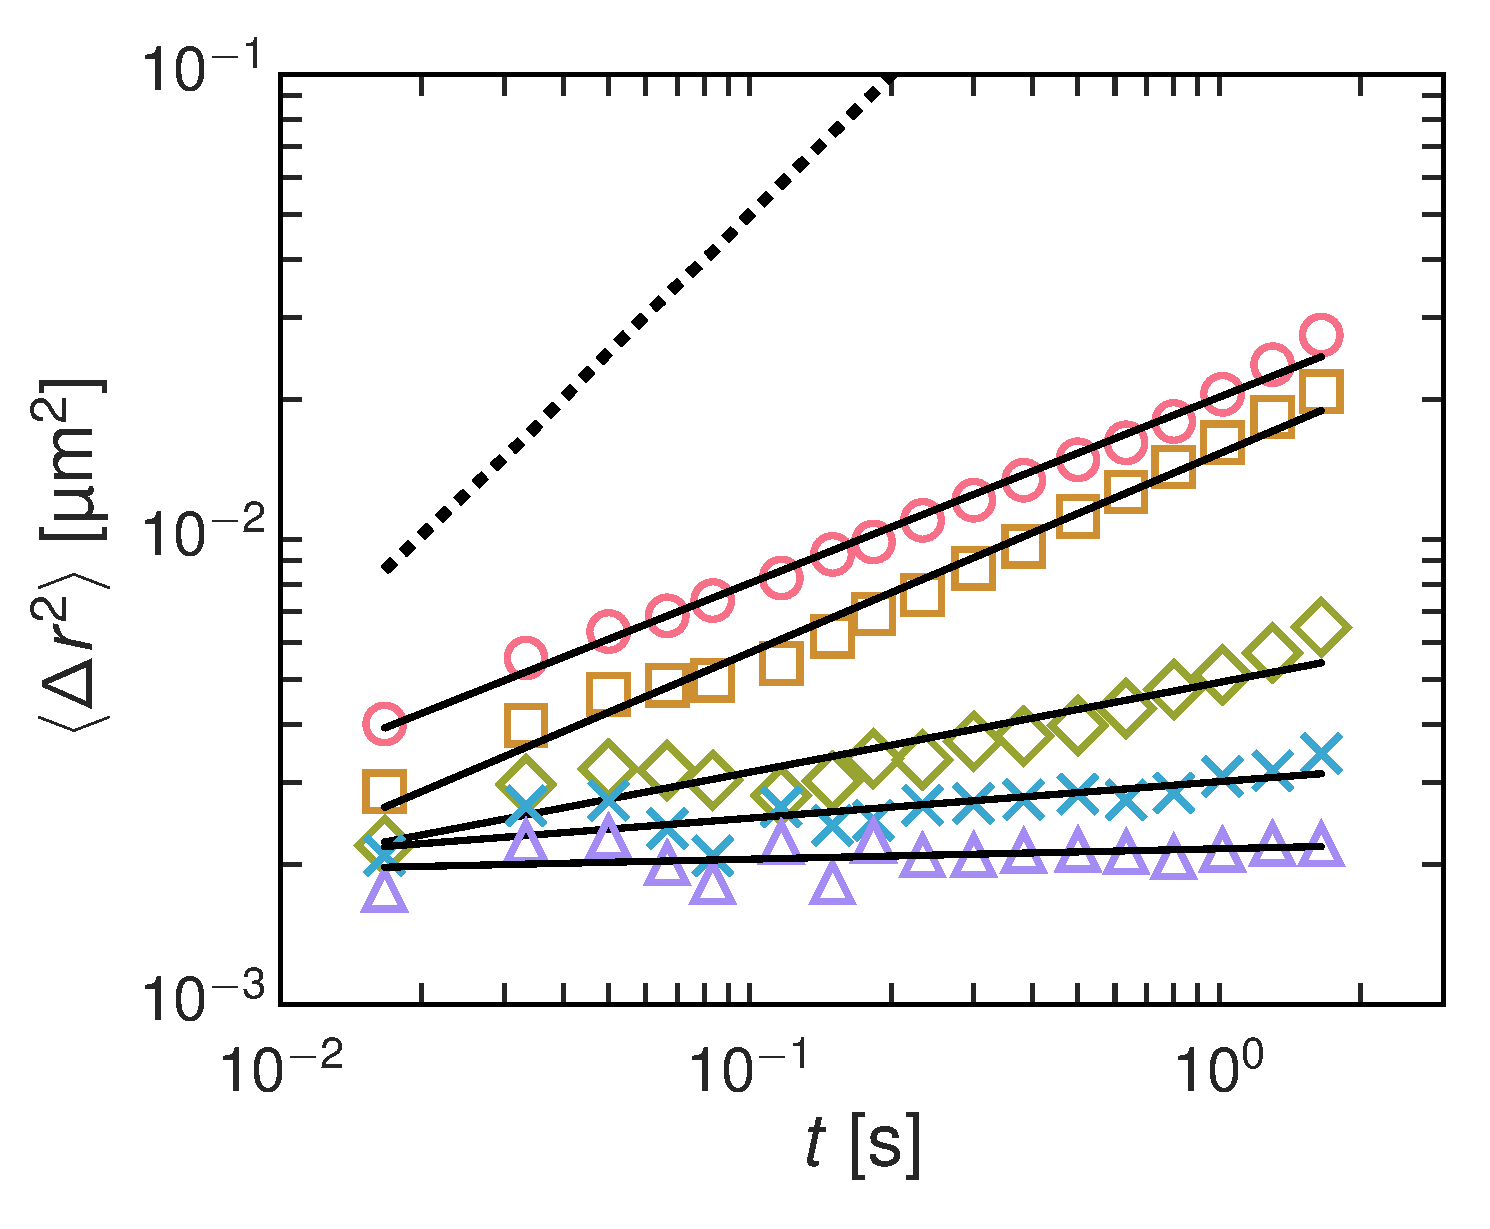
\includegraphics[width=\columnwidth]{bacteria/R7-transition-ensemble-msds}
  \caption{Ensemble-average mean squared displacement of colloids at several ages (red circles: 57 seconds, orange squares: 360, green diamonds: 1080, blue X�s: 10080, purple triangles: 88920) during biofilm formation at an oil-water interface for a trial with no active stage.  For reference, the dashed line displays the mean squared displacement of colloids at the bare oil-water interface in the absence of bacteria.  The solid lines display the result of power-law fits.}
  \label{fig:R7}
\end{figure}

Figure \ref{fig:R7} shows the ensemble-averaged mean-squared displacement $\langle \Delta r^2 (t)\rangle$ of the colloidal probes at several ages ta of biofilm formation following creation of the interface.  Because each mean-squared displacement is determined from 1 minute of video, the maximum lag time t is restricted to $t < 2$ s to assure adequate statistics.  Again for reference, the mean-squared displacement of colloids diffusing at the oil interface of pure Instant Ocean containing no bacteria is also shown.  At our earliest measurement of biofilm formation, the colloidal mean-squared displacement varies sublinearly with lag time, indicating a drag due to the development of a film with viscoelastic character. 

Within the limited dynamic range of accessible lag times, $\langle \Delta r^2 (t)\rangle$ is approximated as a power law, $\langle \Delta r^2 (t)\rangle \sim t^n$, with $n < 1$. As shown in Fig. \ref{fig:R8}, the power-law exponent $n$ decreases steadily with increasing age, signifying increasingly subdiffusive motion. While in principle the probe mobility is affected by both the interfacial film and drag from the surrounding bulk oil and water, given the large difference between $\langle \Delta r^2 (t)\rangle$ in the presence of the forming film and at the neat interface, we can safely infer that the bulk contributions to the drag are insignificant. In this case, under appropriate conditions one can obtain the frequency-dependent interfacial shear modulus, $G^*(\omega) = G'(\omega) + iG''(\omega)$, from the Brownian motion of the probes through a two-dimensional version of a generalized Stokes-Einstein relation, \cite{Helfer2001,Maestro2011}

\begin{equation}
\label{eqn:gse}
G^*(\omega)=\frac{k_B T}{\pi i\omega\mathcal{F}_u\left\{\langle \Delta r^2 (t)\rangle\right\}}
\end{equation}

\noindent where $\mathcal{F}_u\left\{\langle \Delta r^2 (t)\rangle\right\}$ is the unilateral Fourier transform of the mean-squared displacement.  Following Eq. (\ref{eqn:gee}, power-law behavior in the mean-squared displacements of the colloidal probes, $\langle \Delta r^2 (t)\rangle \sim t^n$ with $n < 1$, implies the film�s shear modulus has power-law frequency dependence, $G'(\omega) \sim G''(\omega) ~ \omega n$ \cite{Mason2000}. 

\begin{figure}[htbp]
  \centering
  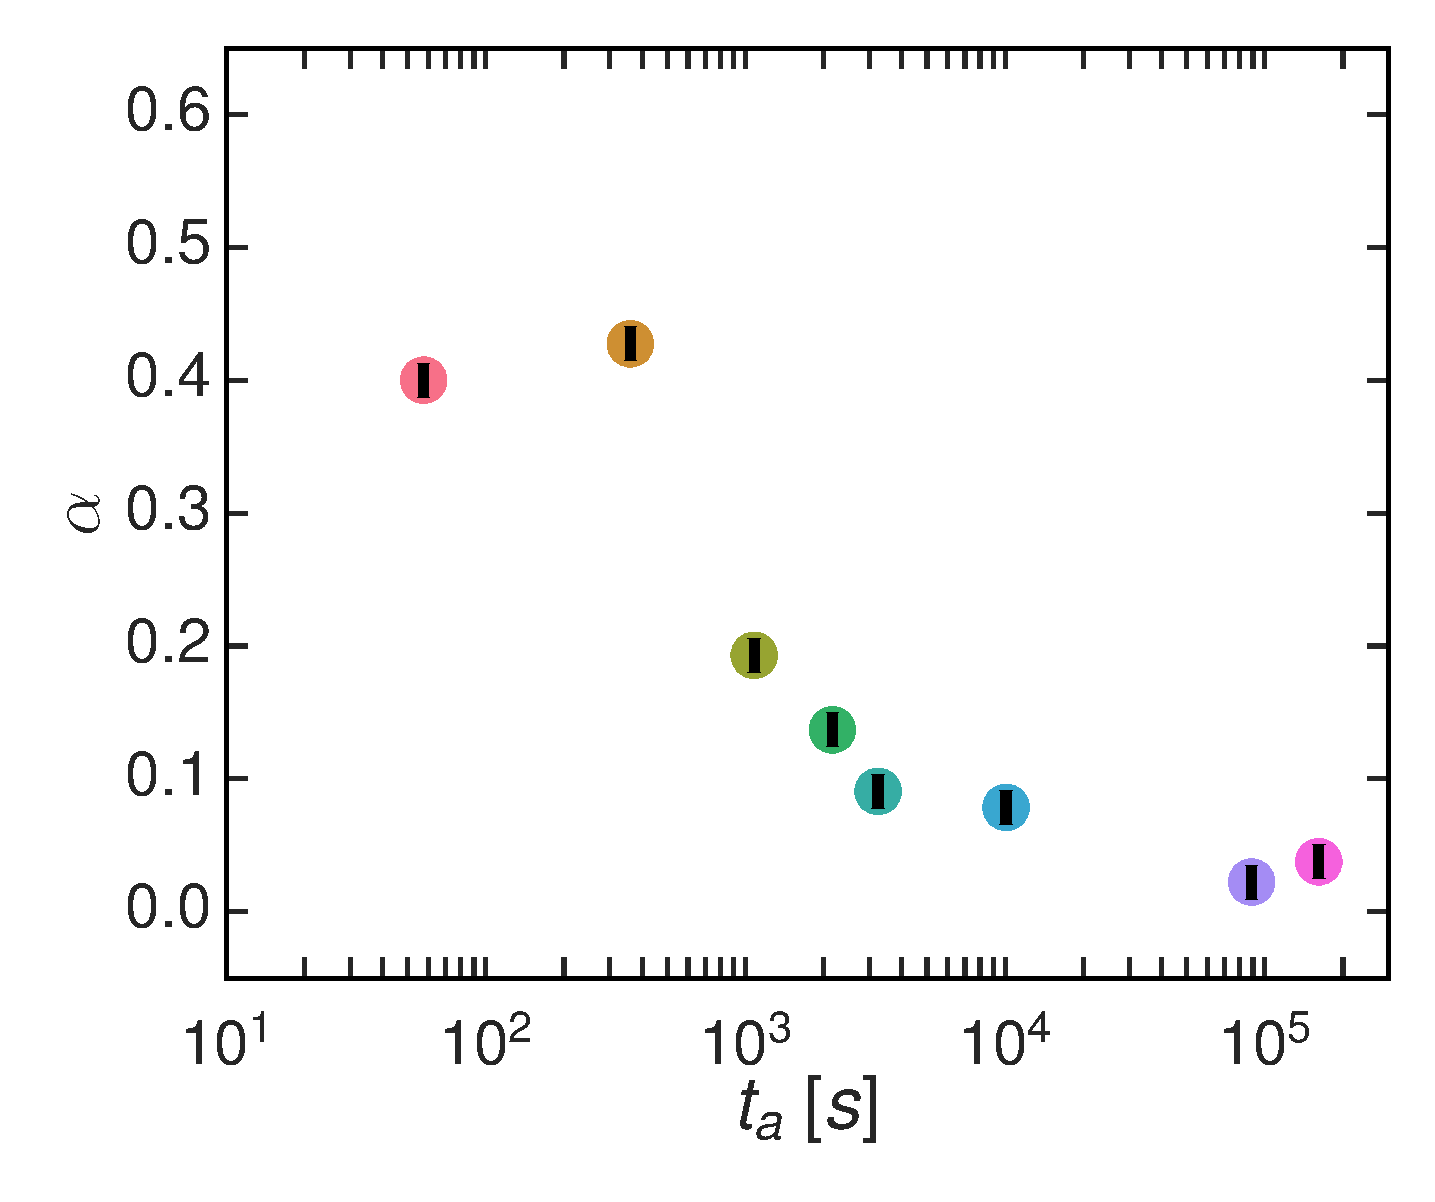
\includegraphics[width=\columnwidth]{bacteria/R8-transition-power-law-exp}
  \caption{Power-law exponent characterizing the ensemble average mean-squared displacements, $\langle \Delta r^2 (t)\rangle \sim t^{\alpha}$, of colloids the oil-bacteria solution interface as a function of the age since formation of the interface.}
  \label{fig:R8}
\end{figure}

\begin{figure}[htbp]
  \centerline{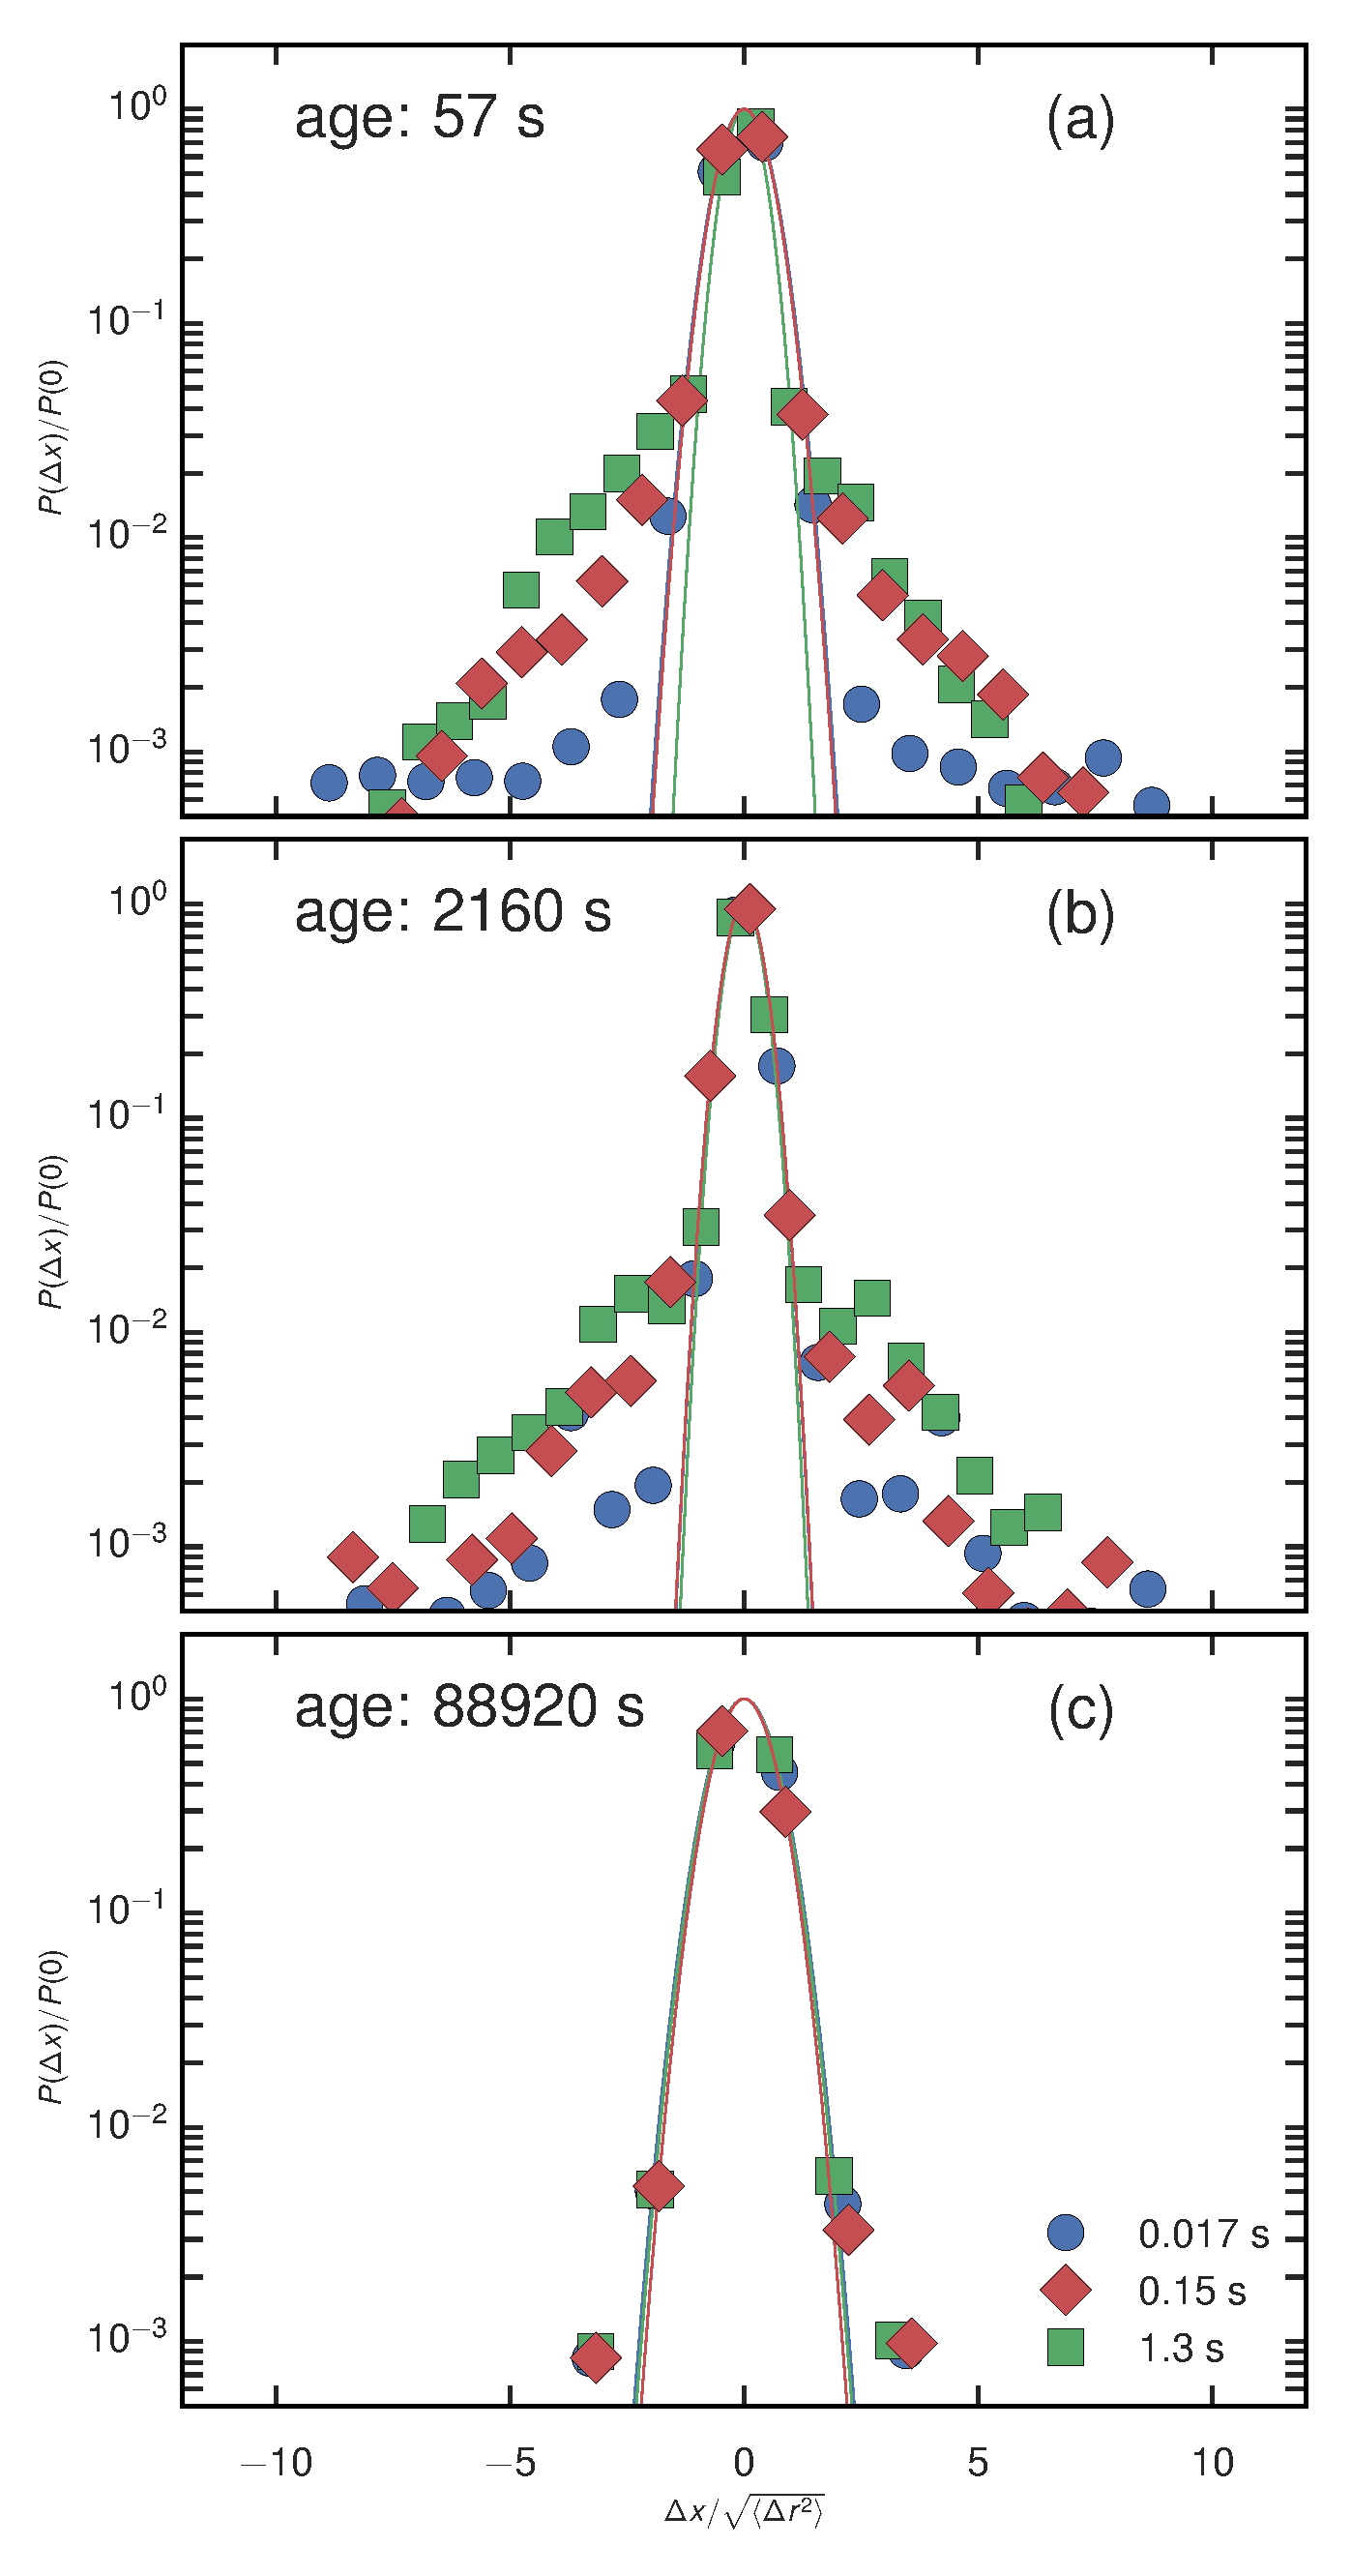
\includegraphics[width=\columnwidth,height=0.8\textheight,keepaspectratio]{bacteria/R9-viscoelastic-transition-vanhove-collapse}}
  \caption{Normalized probability distribution functions for colloidal displacements at lag times of 0.016 s (blue), 0.15 s (green), and 1.3 s (red) at film ages (a) 57 s, (b) 2160 s, and (c) 88920 s during the viscoelastic stage of biofilm formation.  The solid lines display the results of fitting Gaussian lineshapes in the regions of the peaks of the distributions, highlighting the enhanced, non-Gaussian probability for large displacements.}
  \label{fig:R9}
\end{figure}

Such weak power-law frequency dependence of $G^*(\omega)$ is characteristic of the rheology of a broad range of disordered complex fluids including concentrated microgel solutions\cite{Ketz1988}, foams, \cite{Khan1988} paint, \cite{Mackley1994} intracellular matrix,\cite{Fabry2001} compressed emulsions, \cite{Mason1995}  clay suspensions, \cite{Bonn2002} and liquid-crystal nanocomposites \cite{Bandyopadhyay2005} and is indicative of a broad spectrum of relaxation times.  In most cases, the power-law exponent typically lies in the range $n\approx$ 0.1 to 0.3.  The soft glassy rheology model \cite{Sollich1998} explains this response as a general consequence of structural disorder and metastability, and provides a unifying theoretical framework for this behavior.  In this model, $n$ serves as an effective noise temperature, with systems approaching a glass transition as $n\rightarrow 0$.  Thus, the steady decrease in $n$ with layer age reported in Fig. \ref{fig:R8} points to increasingly glassy dynamics characterizing the structural response of the biofilm.  
An important property of soft glassy systems is their non-equilibrium behavior and spatial heterogeneity.  As a measure of these features, Figs. \ref{fig:R9}(a)-(c) show the PDFs of colloidal displacements at three ages during the viscoelastic transition.  In each case, the PDF is shown at three lag times normalized by the mean-squared displacement at that lag time.  At the earlier two ages, ($t_a$ = ??? and ???), during which the viscoelastic character of the film is evolving rapidly, the PDFs show a pronounced non-Gaussian components corresponding to enhanced probability of large displacements.  These non-Gaussian contributions resemble those characterizing the colloidal dynamics in the active stage (Figs. \ref{fig:R3} and \ref{fig:R4}); however, their origin in this case is different.  Unlike at the active interface, the perturbations here are thermal, and each individual particle�s displacements are Gaussian.  The non-Gaussian distributions result from variation in the mobility of different particles, evincing a spatially heterogeneous interface of rheological microenvironments \cite{Valentine2001}.  Surprisingly, this heterogeneity diminishes at late ages, as illustrated by the closer-to-Gaussian distributions in Fig. \ref{fig:R9}(c), when the interface�s evolution has slowed and the film is nearly elastic.  An interesting future study would be to compare this spatial heterogeneity with that of films formed in the presence of an extended stage of activity by swimming bacteria to investigate the role of biomixing in suppressing such heterogeneity. 
 